\documentclass{article}


%% We should use this latex document to store all the figures and
%% tables, and then do "make" to generate the floats.pdf which we will
%% send along with the main manuscript text.
\usepackage[a4paper,margin=2cm]{geometry}
\usepackage{graphicx}
\usepackage{mathpazo}
\usepackage{tabularx}
\usepackage[table]{xcolor} 

\begin{document}
\pagestyle{empty}


%% One float per page:
%% http://tex.stackexchange.com/questions/22191/forcing-a-figure-strictly-on-a-separate-page
\makeatletter
\@fpsep\textheight
\makeatother

\begin{figure}
  \centering
  \fbox{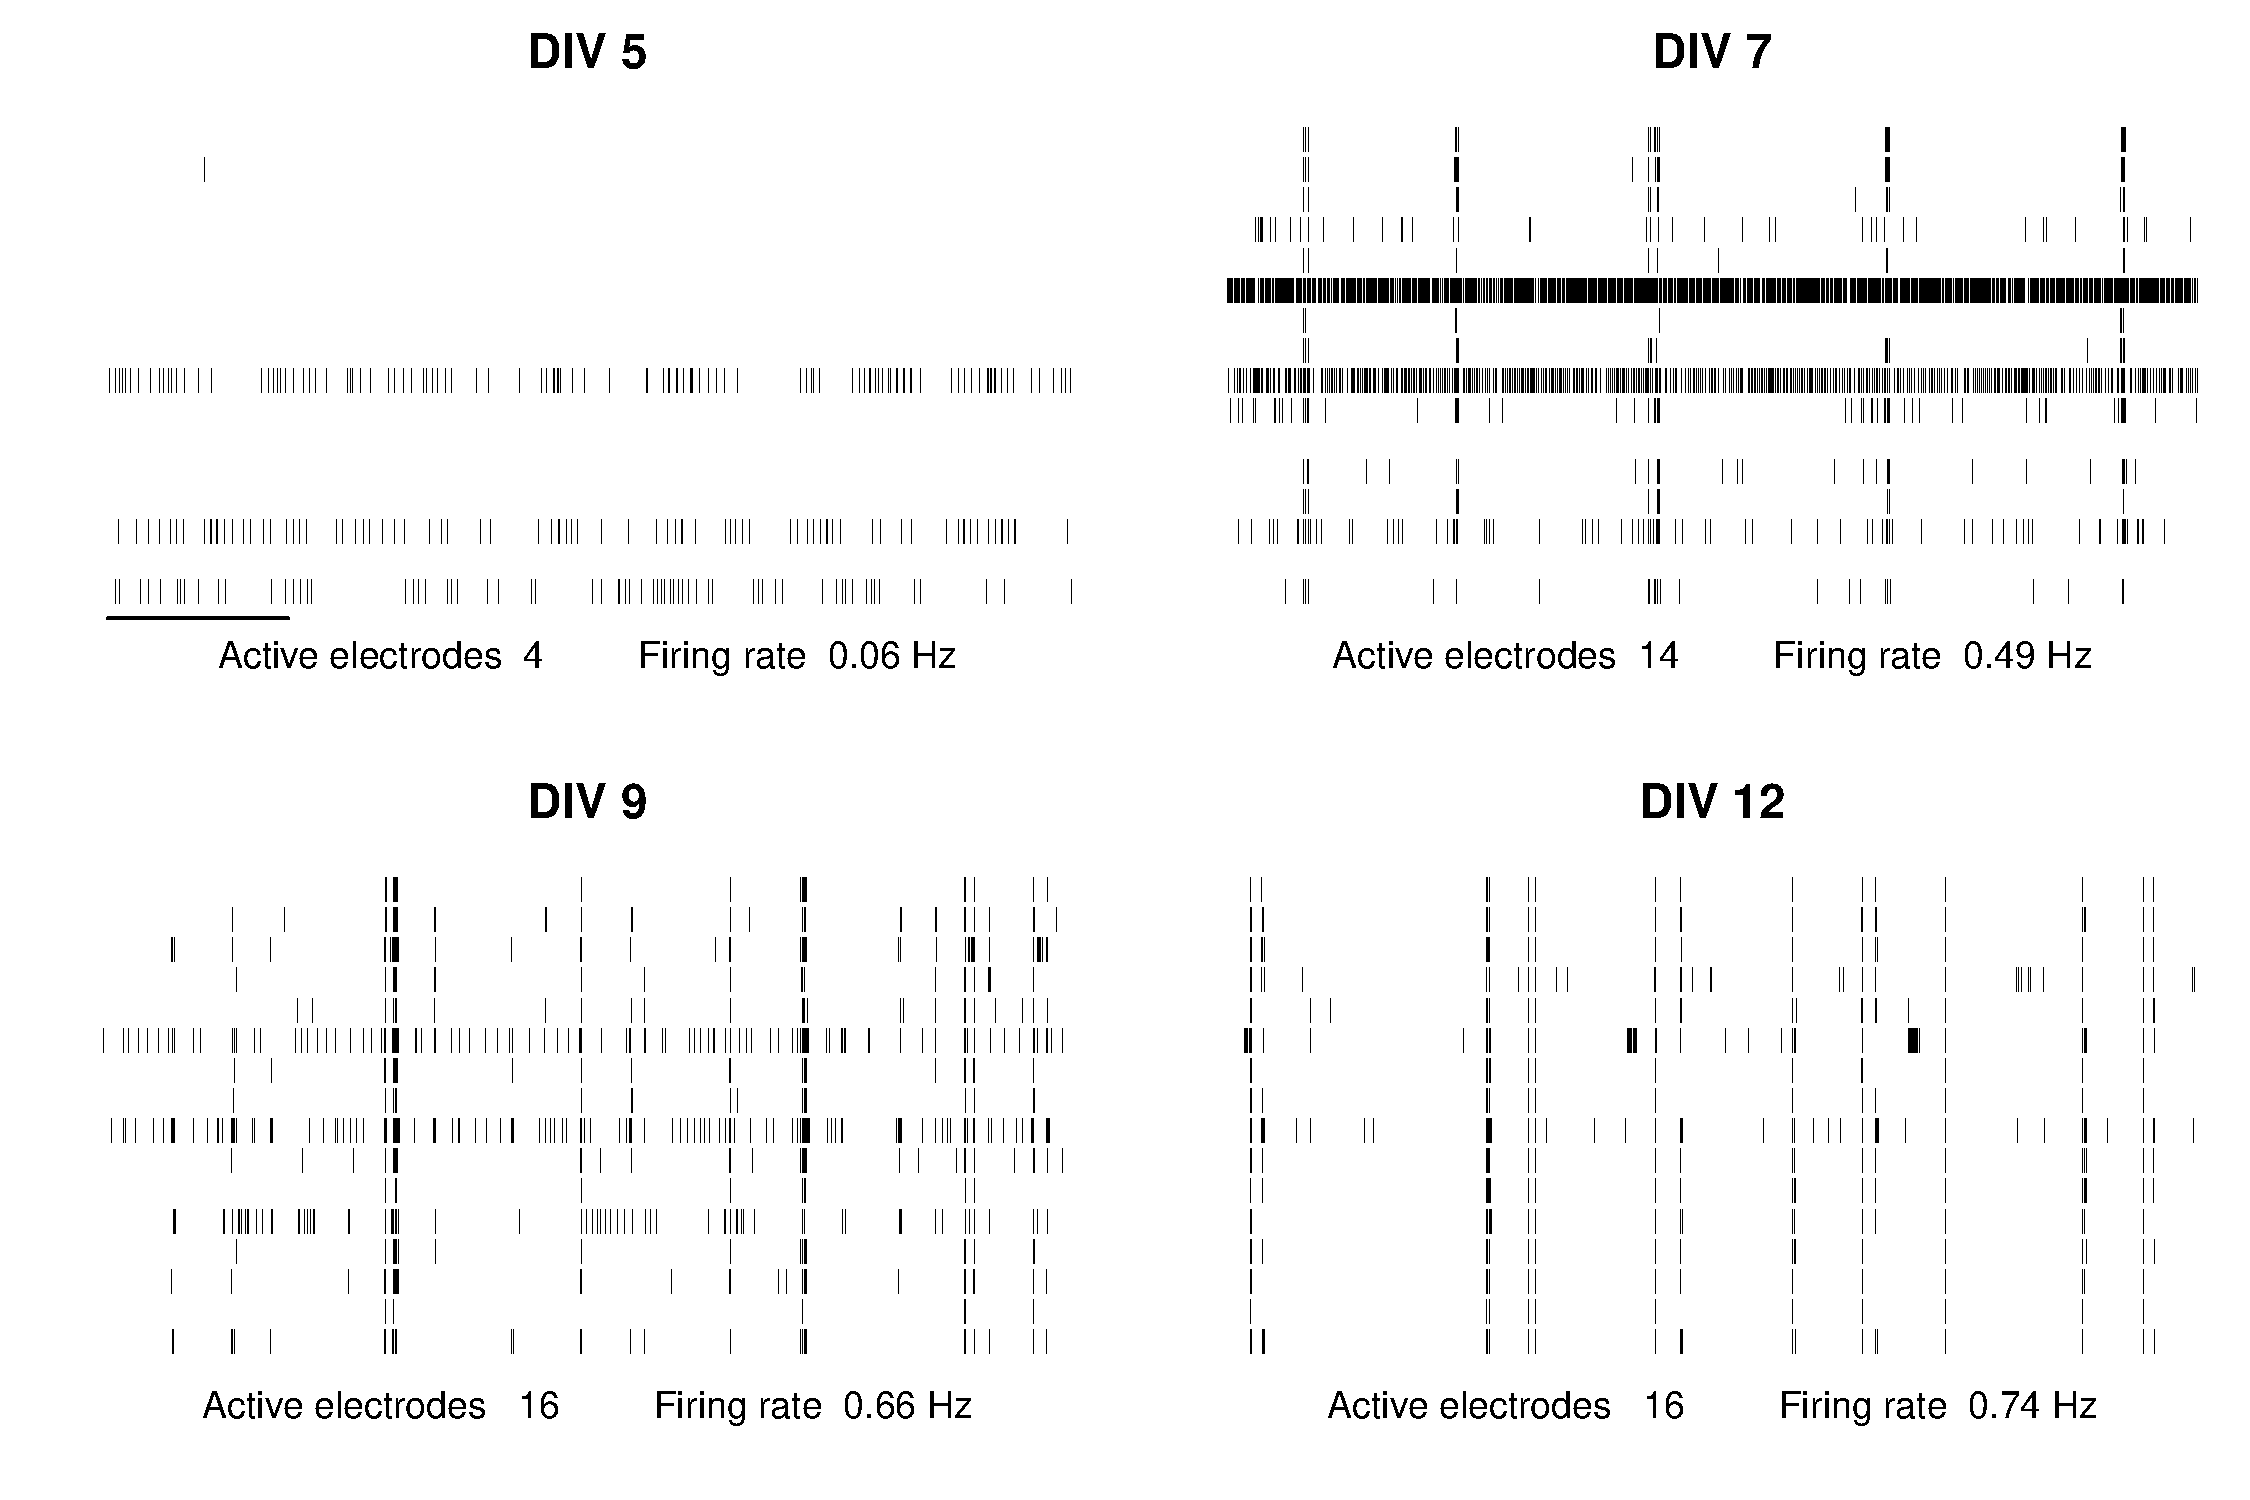
\includegraphics[width=170mm]{rasters.pdf}}
  \caption{Example raster plots from the same well over the four
    developmental ages (days in vitro, DIV) studied. Each row
    represents the spike train from one electrode. The scale bar for
    all raster plots is 60s.}
\end{figure}

\begin{figure}
  \centering
  \fbox{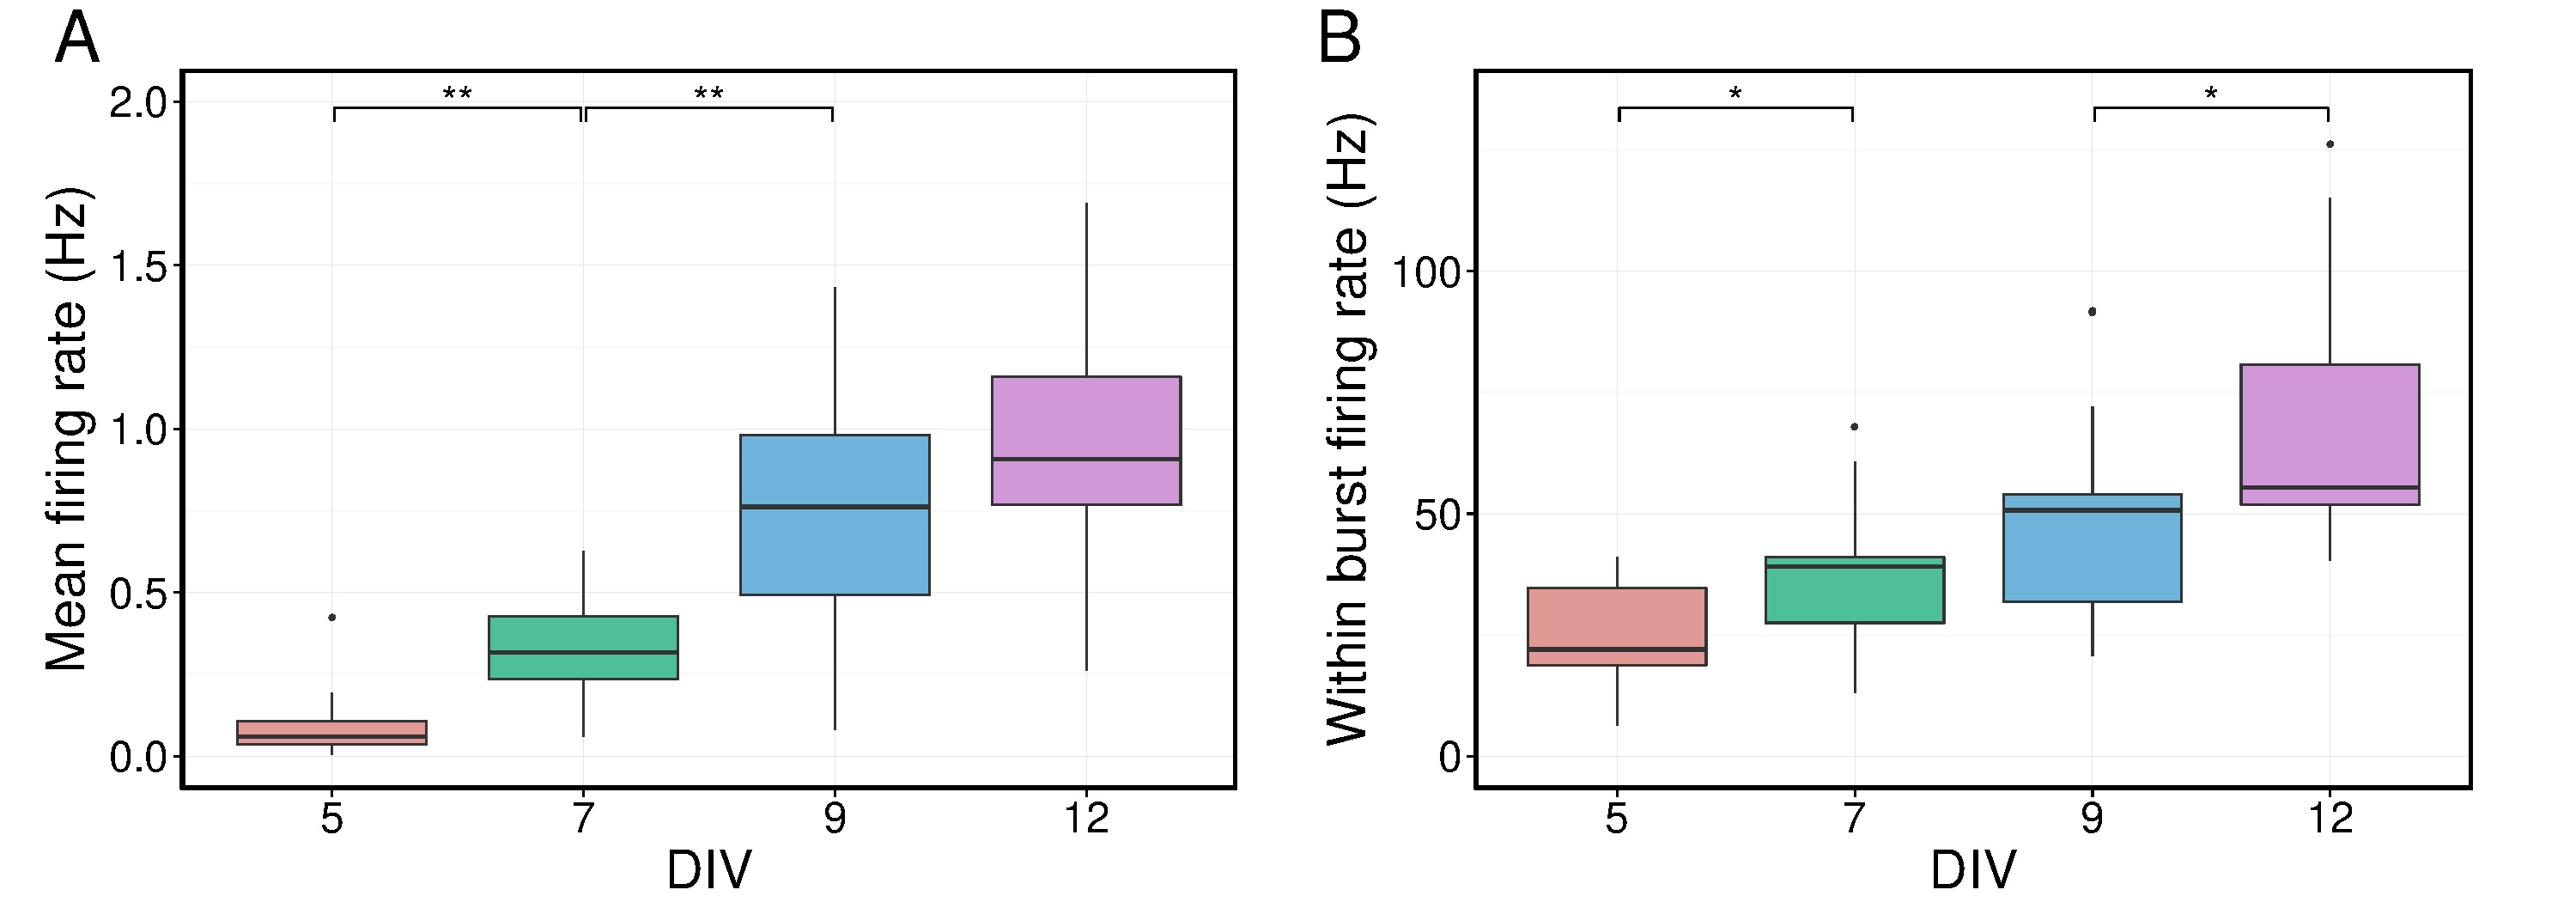
\includegraphics[width=170mm]{firingrate.pdf}}
  \caption{Mean firing rate (A) and within burst firing rate (B)
    increase with development.  Box plots showing median and
    interquartle range are shown for n=16 plates. Stars represent significant difference in median values between pairs of consecutive ages at the 0.05 level. P-values obtained from a Mann-Whitney test, corrected for multiple comparisons using the false discovery rate method.}
\end{figure}

\begin{figure}
  \centering
  \fbox{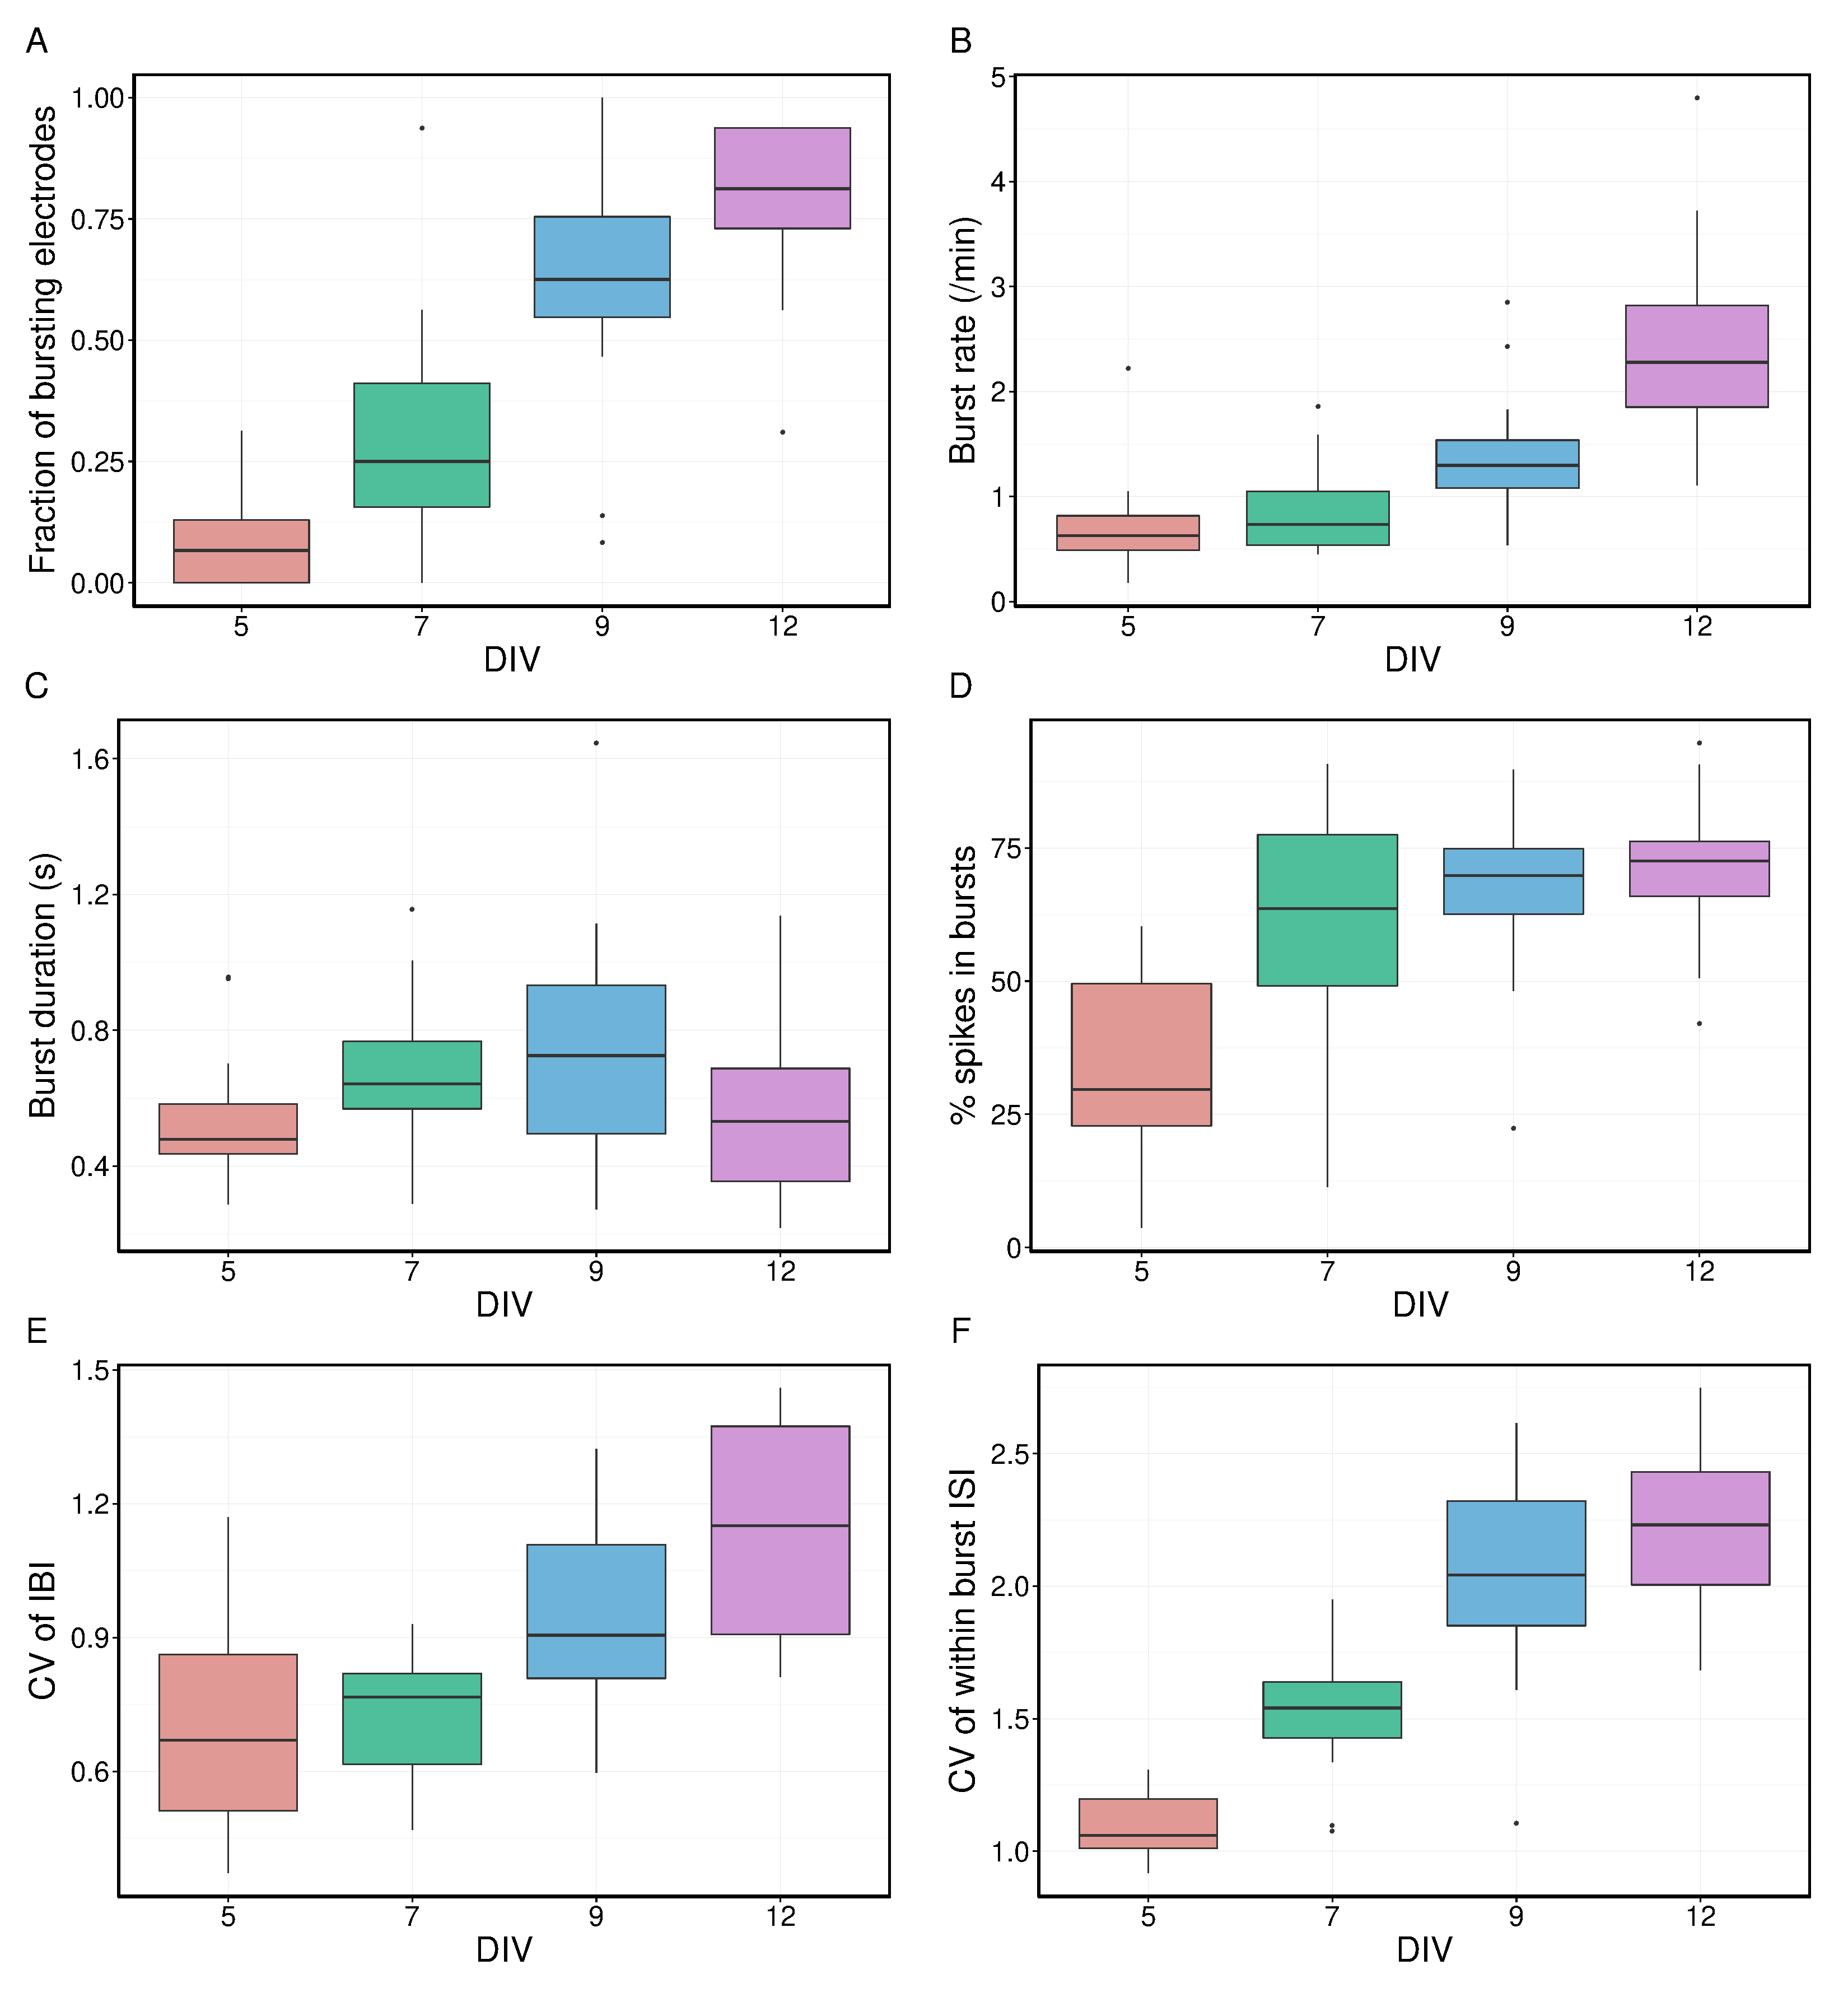
\includegraphics[width=170mm]{bursts.pdf}}
  \caption{Bursting properties of spontaneous activity mature with
    development.  Each panel shows box plots of one burst feature
    across development. A: Bursts
    per minute. B: Burst duration. C: Fraction of bursting electrodes. D: Percentage of spikes in
    bursts.  E: Coefficient of variation (CV) of interburst interval
    (IBI).  F: CV of within burst interspike interval (ISI). Stars represent significant difference in median values between pairs of consecutive ages at the 0.05 level. P-values obtained from a Mann-Whitney test, corrected for multiple comparisons using the false discovery rate method.}
\end{figure}

\begin{figure}
  \centering
  \fbox{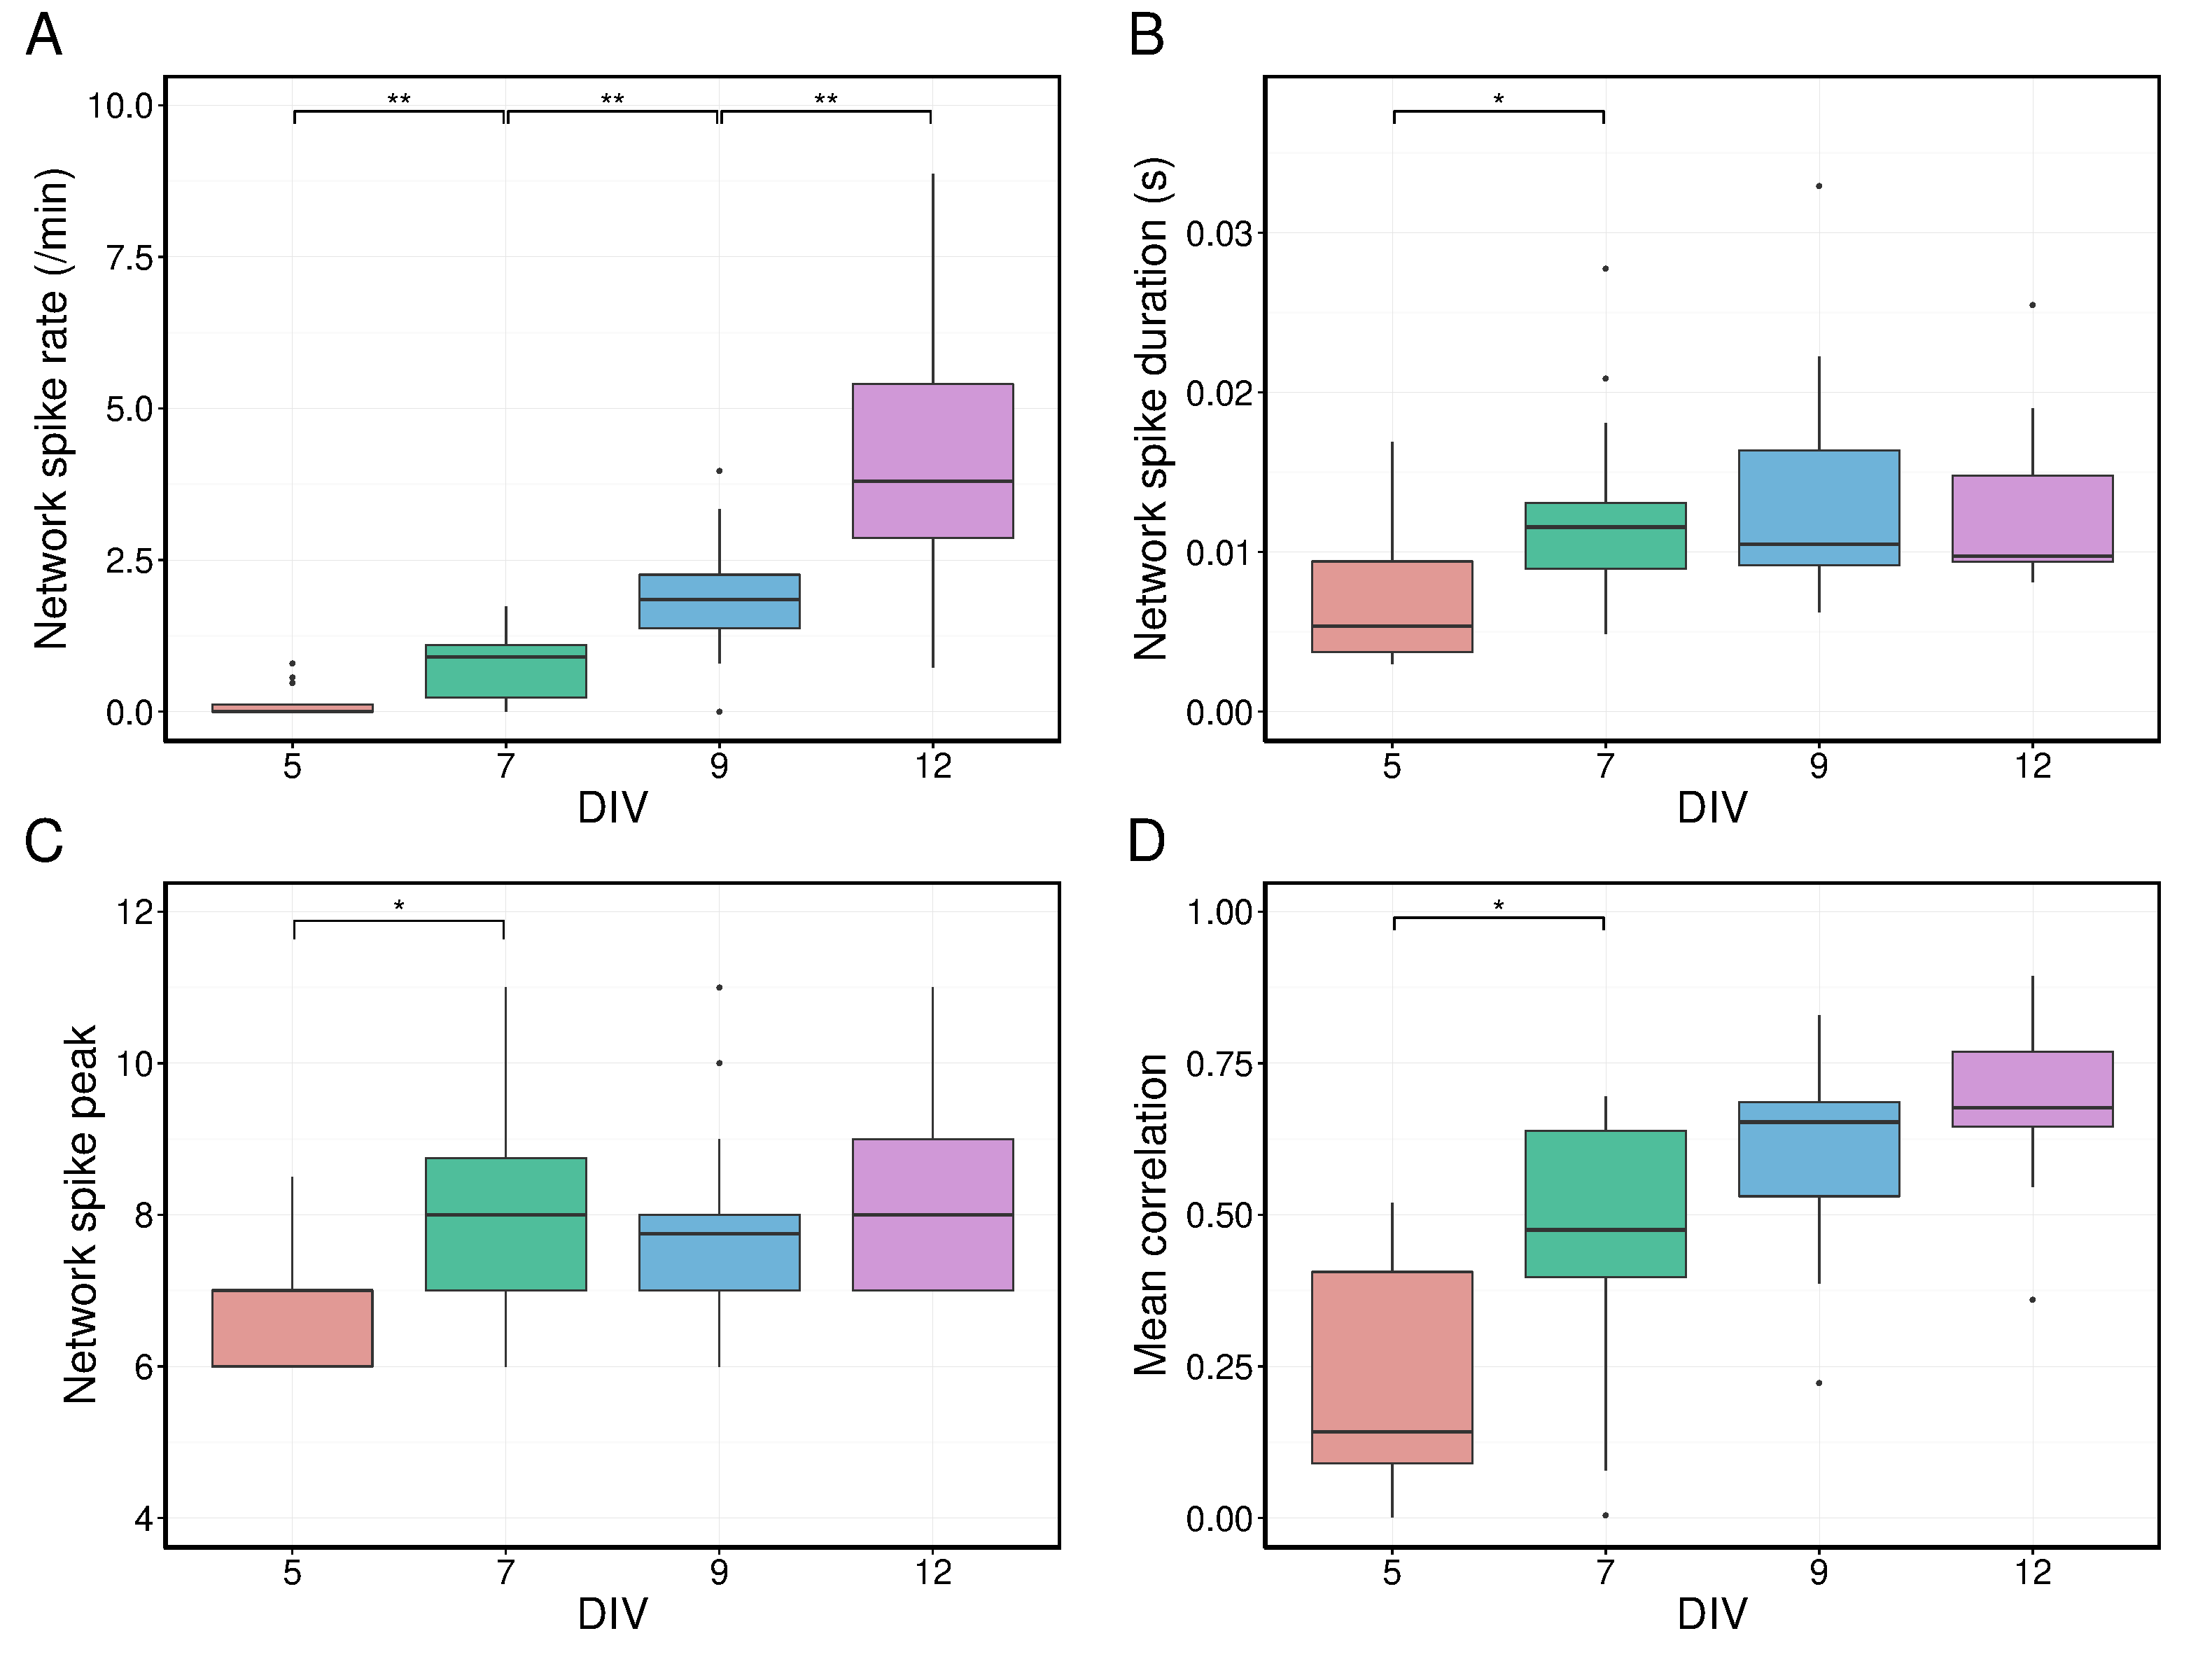
\includegraphics[width=170mm]{ns.pdf}}
  \caption{Network properties of spontaneous activity assessed
    across development.  A: Network spike rate.  B: Network spike
    duration.  C: Network spike peak. D: Mean pairwise correlation. Stars represent significant difference in median values between pairs of consecutive ages at the 0.05 level. P-values obtained from a Mann-Whitney test, corrected for multiple comparisons using the false discovery rate method.}
\end{figure}

\begin{figure}
  \centering
  %%\fbox{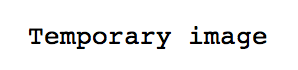
\includegraphics{temp.png}}
  \fbox{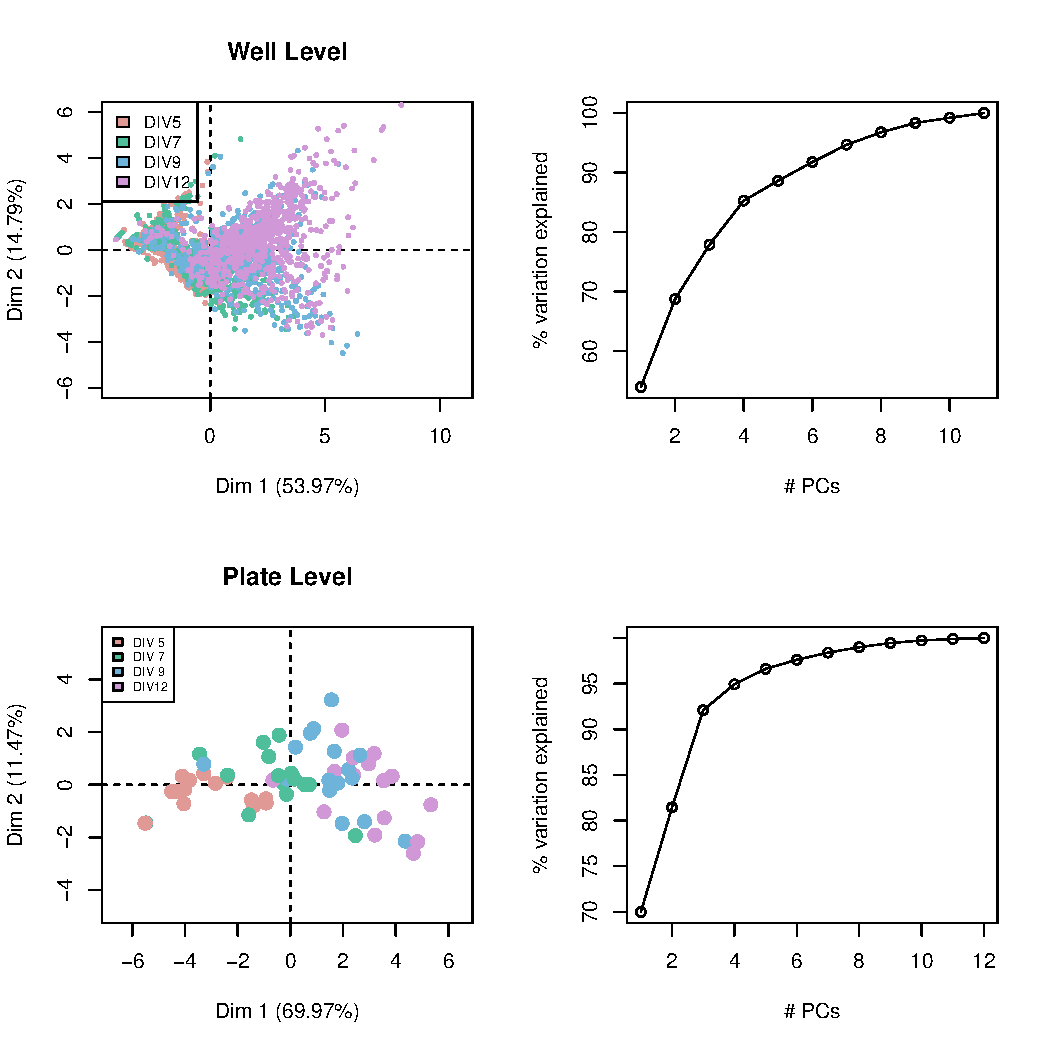
\includegraphics{../Analysis/4_in_1.pdf}}
  \caption{[Top left] Well-level PCA projection of 12-dimensional
feature vectors onto PC dimension 1 (x-axis) and 2 (y-axis).  Each dot
represents a well, colored by day in vitro (DIV) of recording. Rough
ordering from youngest (red, DIV 5) to oldest (purple, DIV 12)
wells is apparent in change of colors along the positive direction
. (Top right) Scree plot displays \% variance explained by the number
of PC dimensions. [Bottom left] Plate-level PCA projection of plate
averages onto PC dimension 1 (x-axis) and 2 (y-axis).  As in top,
rough ordering of observations by DIV is apparent in the red to purple
transition along the x-axis. (Bottom right) Scree plot of plate-level
PCA. Compared to the well-level PCA scree plot, a larger amount of
variation is captured in the first two PC dimensions indicating that
well averaging reduces variability.
}
\end{figure}

\begin{figure}
  \centering
   \fbox{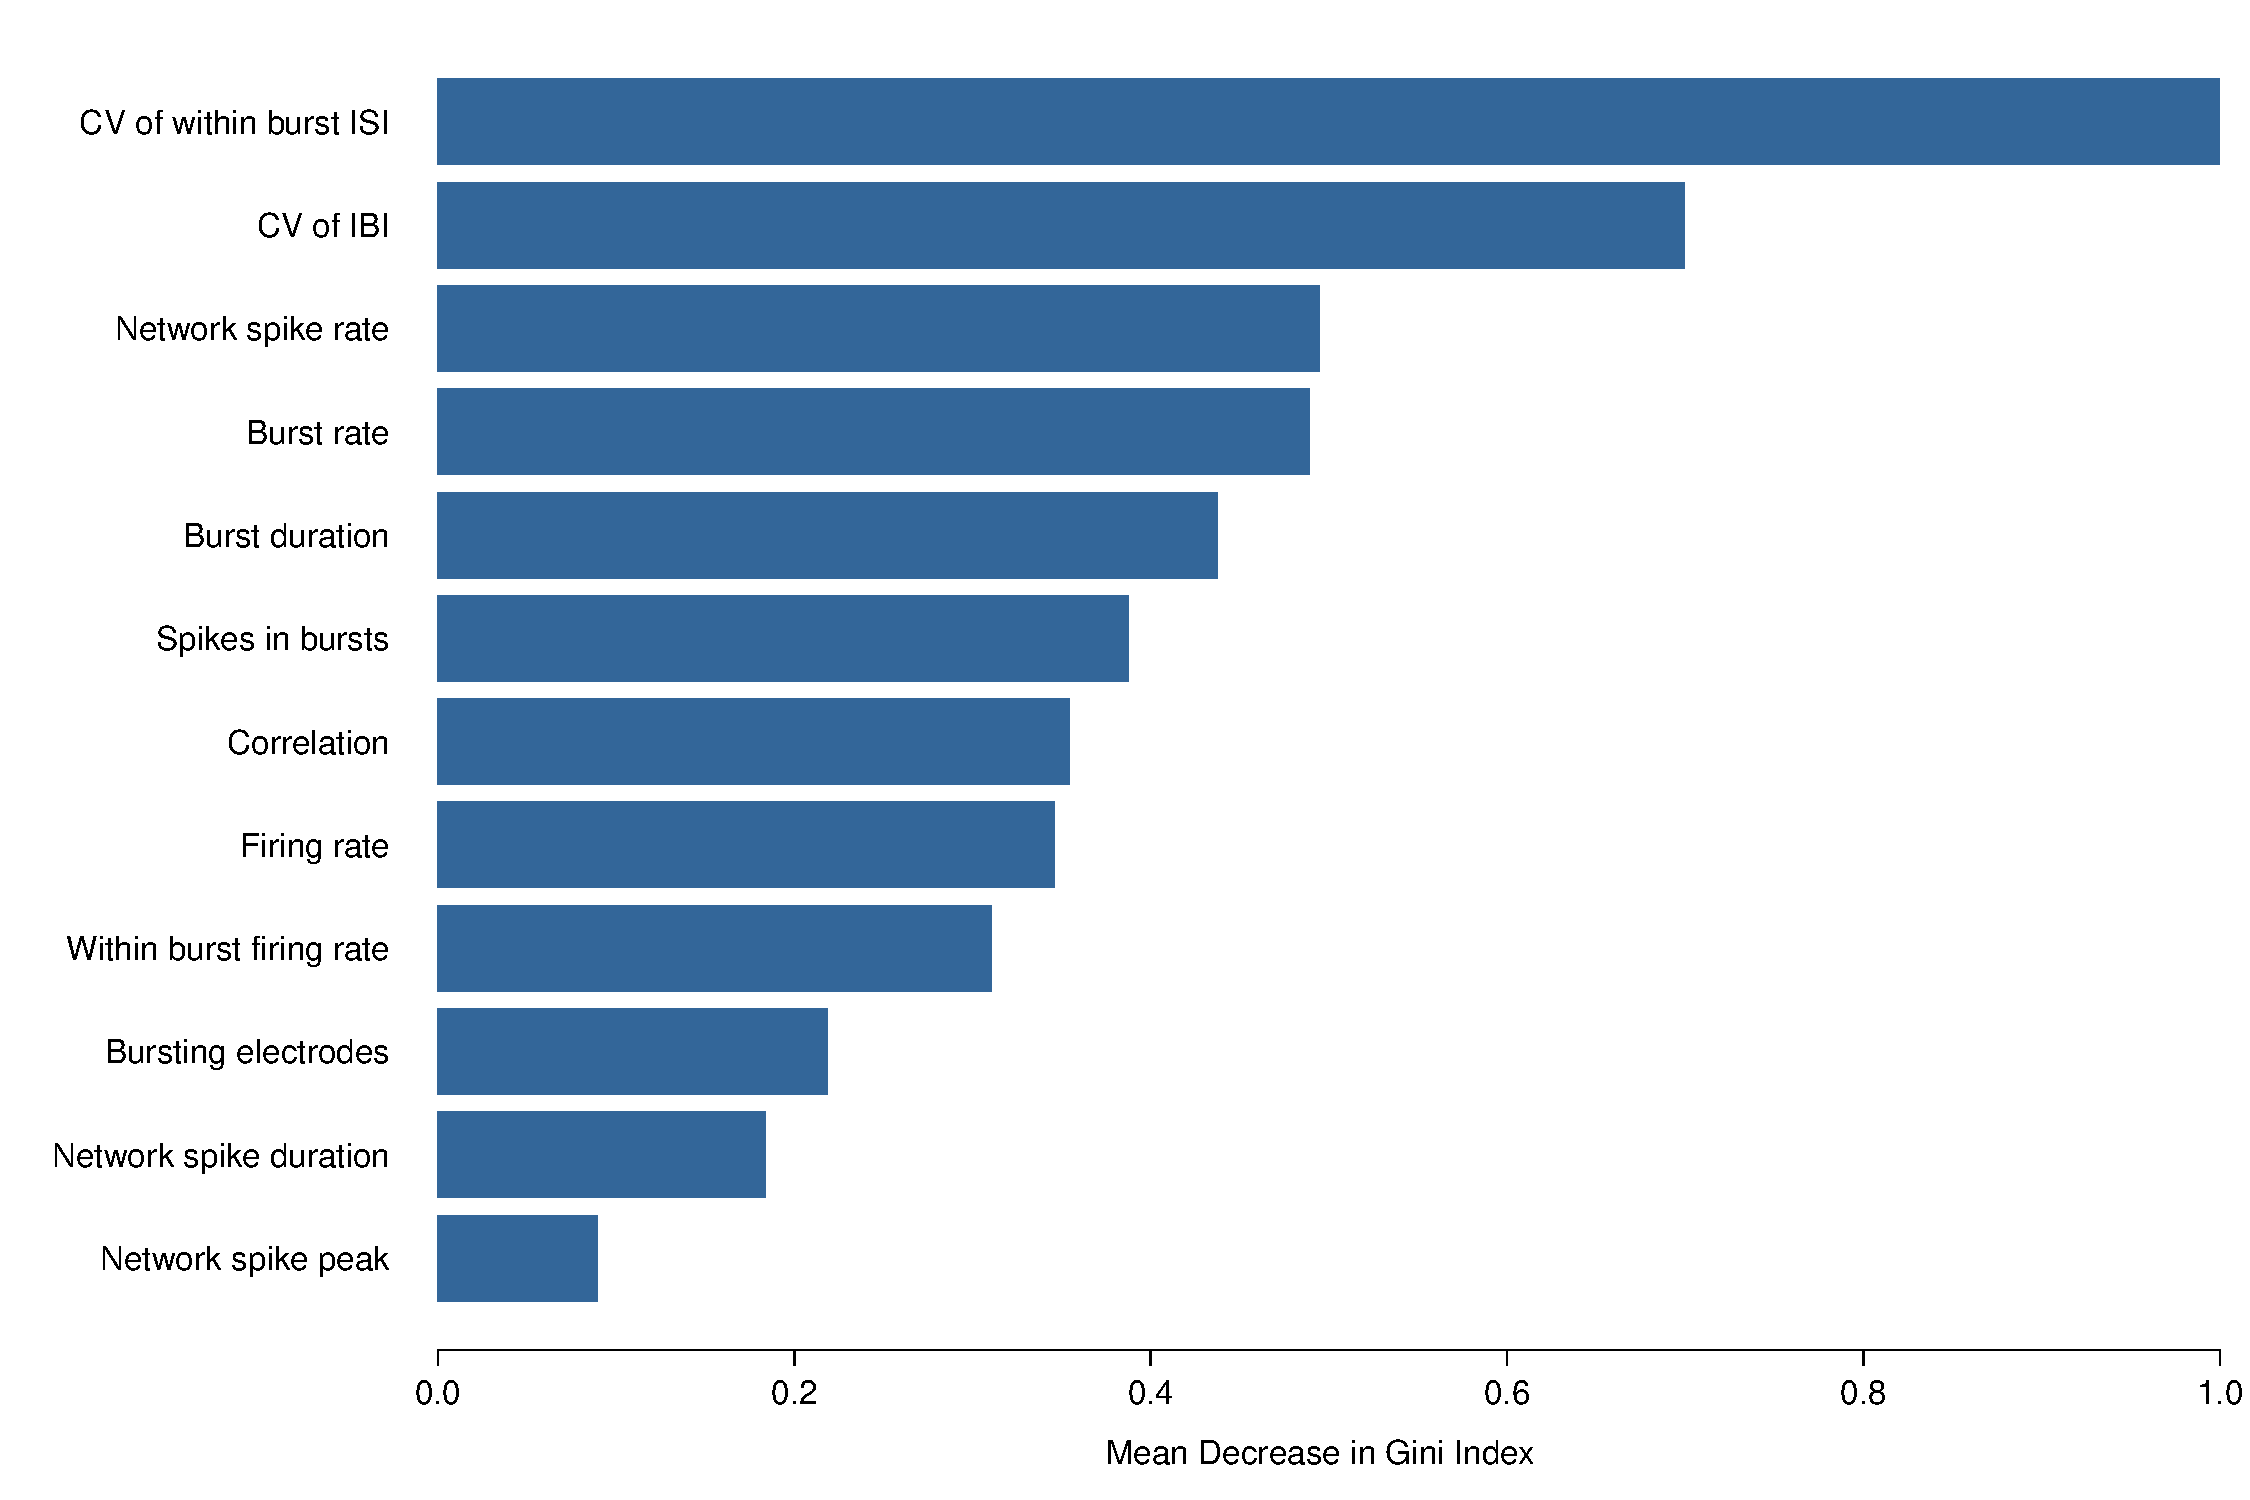
\includegraphics[width=170mm]{importance.pdf}}
  \caption{Average importance of features in driving classification,
    relative to the most important feature.}
\end{figure}

\begin{figure}
  \centering
  \fbox{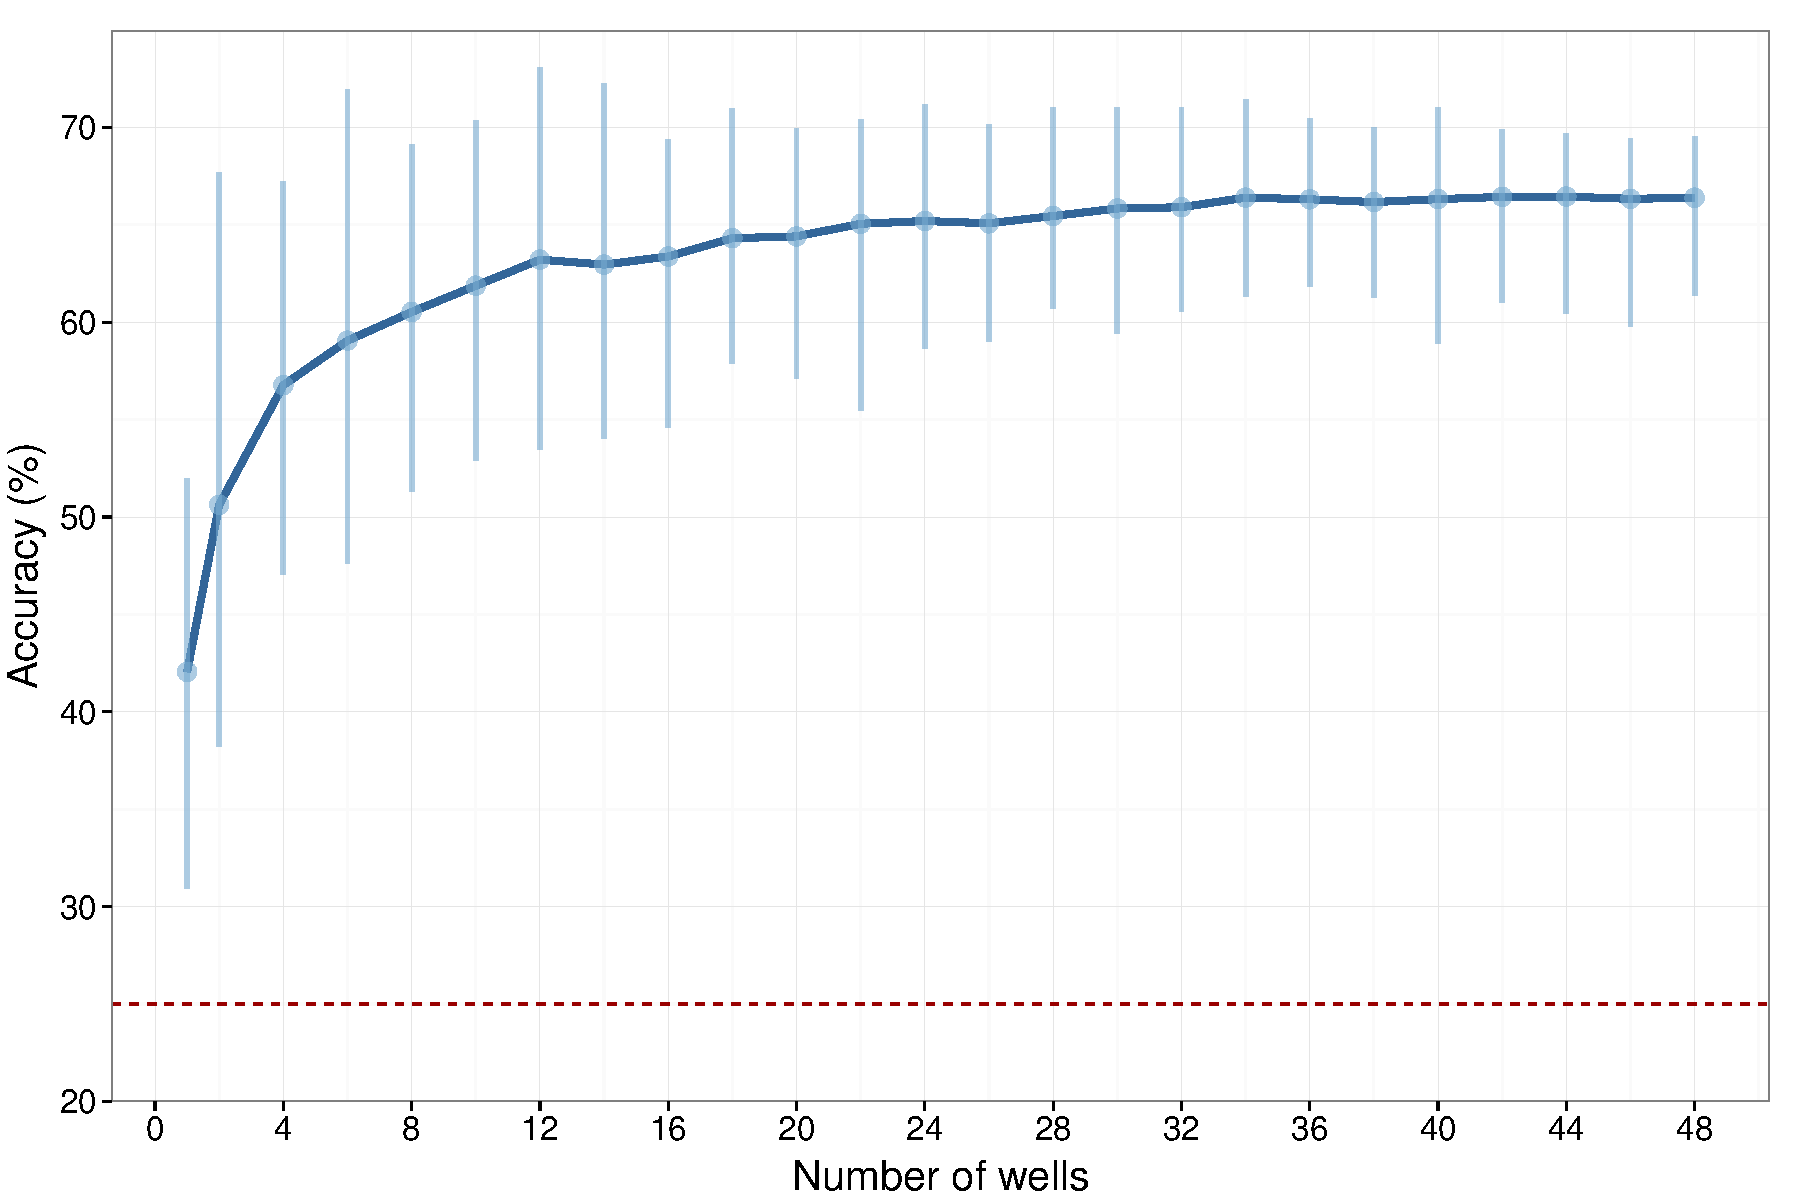
\includegraphics[width=170mm]{accuracy.pdf}}
  \caption{Accuracy of predicting the age of each well by sampling
    $n \leq 48$ wells on each plate. Dark blue line shows the mean
    accuracy, while the vertical lines show the minimum and maximum
    accuracy over 100 trials with random choices of wells.  For
    $n=48$, the error bars indicate the small variability in
    classification due to the partioning of data into train/test sets.
    The red dotted line indicates baseline level of performance (25\%)
    for a classifier.}
\end{figure}

\begin{table}
  \centering
  \rowcolors{1}{white}{gray!25}
  	\begin{tabular}{|l|m{11cm}|}
  		\hline
  		Feature & Description
  		\\ \hline 
  		Mean firing Rate & The mean firing rate (MFR) on each electrode was calculated. The well value was the median value of all active electrodes. 
  		\\ Burst rate  & The number of bursts per minute on an electrode was calculated. The well value was the median value from all electrodes that exhibited bursting behaviour. 
  		\\ Burst duration  & The mean duration of all bursts on an electrode over the recording period was calculated. The well value was the median value from all electrodes that exhibited bursting behaviour.
  		\\ Fraction of bursting electrodes  & An electrode was classified as bursting if the burst rate on the electrode was at least one per minute. The well value was the number of electrodes classified as bursting as a fraction of the total number of active electrodes on the well.  
  		\\ Within burst firing rate   & The electrode value was the mean firing rate within all bursts on the electrode. The well value was the median value from all electrodes that exhibited bursting behaviour. 
  		\\ Percentage of spikes in bursts & The number of spikes on an electrode classified as being within bursts divided by the total number of spikes on the electrode. The well value was the median value from all electrodes that exhibited bursting behaviour.  
  		\\ CV of IBI & The ratio of the standard deviation to the mean of the length of all inter-burst intervals (IBI) on an electrode. The well value was the median value from all electrodes that exhibited bursting behaviour.  
  		\\ CV of within burst ISIs &  The ratio of the standard deviation to the mean of the length of all inter-spike intervals (ISI) within bursts on an electrode. The well value was the median value from all electrodes that exhibited bursting behaviour.  
  		\\ Network spike rate &  The well value was the number of network spikes on the well per minute of the recording period (See Methods section for definition of a Network Spike).
  		\\ Network spike duration  & The duration of a network spike was defined as the length of time during which the number of active electrodes on the well exceeded the threshold value (5). The well value was taken as the median duration of all network spikes on the well during the recording period.
  		\\ Network spike peak  & The maximum number of active electrodes during each network spike. The well value was taken as the median peak value of all network spikes on the well during the recording period. 
  		\\ Mean correlation & The correlation between every pairwise combination of electrodes on a well was calculated using the spike time tiling coefficient (Cutts \& Eglen, 2015) with $\Delta t = 50ms$. (See Methods section for definition). The well value was the mean of the pairwise correlations between all distinct electrodes on the well. 
  		\\ \hline
  	\end{tabular}
  \caption{Features used in our analysis and a brief description of how
    they were calculated.}
\end{table}

\begin{table}
  \centering
  \rowcolors{2}{white}{gray!25}
  \begin{tabular}{|l|c|}
  	\hline
  	\textbf{Feature} & \textbf{Accuracy \%}
  	\\ \hline 
  	CV of within burst ISI & 49.2
  	\\CV of IBI & 58.3
  	\\ Network spike rate& 62.0
  	\\ Burst rate & 65.0
  	\\ Burst duration& 66.0
  	\\ \% Spikes in bursts & 68.3
  	\\Correlation & 69.5
  	\\Firing rate & 71.4
  	\\Within burst firing rate & 72.7
  	\\Bursting electrodes & 73.0
  	\\ Network spike duration & 73.5
  	\\Network spike peak & 73.4
  	\\ \hline
  \end{tabular}
  \caption {Classifier performance at predicting the age of
arrays. Features are listed in decreasing order of importance, and the
value in each row $n=1 \ldots 12$ is the mean percentage of correct
classifications using the top $n$ features.  For example, row 4 shows
that the classifier was 65.0\% accurate at predicting age using the
top four features. }
\end{table}

\begin{table}
  \centering
  \rowcolors{2}{gray!25}{white}
  \begin{tabular}{|l|c|c|c|c|c|c|}
	  \hline
	  \textbf{Feature} & \multicolumn{5}{c}{\textbf{Accuracy \%}} & 
	  \\ \hline
	  & 5 vs 7 & 5 vs 9 & 5 vs 12 & 7 vs 9 & 7 vs 12 & 9 vs 12
	  \\ \hline 
		CV of within burst ISI & 75.0 & 87.5 & 91.8 & 69.9& 78.1 & 57.4
		\\ CV of IBI & 77.4 & 89.5 & 93.6 & 76.8 & 85.5 & 64.7
		\\ Network spike rate& 79.3 & 90.3 & 95.5  & 79.6 & 88.0 & 68.7
		\\ Burst rate & 79.3 & 90.3 & 95.3 & 81.0 & 88.4 & 72.8
		\\ Burst duration& 79.7 & 90.8 & 95.3 & 81.0 & 88.6 & 74.0
		\\ \% Spikes in bursts & 81.6 & 91.3 & 95.6 & 81.5 & 90.4 & 76.4
		\\ Correlation & 82.2 & 92.1 & 95.6 & 82.3 & 90.9 & 77.1
		\\ Firing rate & 82.3 & 91.7 & 95.7 & 82.3 & 90.9 & 80.2
		\\ Within burst firing rate & 84.2 & 92.7 & 96.2 & 82.4 & 91.3 & 81.2
		\\ Bursting electrodes & 83.6 & 92.5 & 96.2 & 82.6 & 91.8 & 81.5
		\\ Network spike duration & 83.7 & 92.9 & 96.8 & 82.9 & 92.8 & 82.0
		\\ Network spike peak & 82.2 & 92.5 & 96.8 & 82.6 & 93.0 & 82.1
	\\ \hline
\end{tabular}
  \caption{Classifier performance at predicting the age of arrays for
    each pairwise combination of ages (days in vitro). Features are listed in
    decreasing order of importance, and the value in each row
    $n=1 \ldots 12$ is the mean percentage of correct classifications using
    the top $n$ features, as described in Table~2.}
\end{table}



\end{document}
